\documentclass[11pt]{book}

\usepackage[italian]{babel}
\usepackage{graphicx}
\usepackage{verbatim}
\usepackage{fancyvrb}
\usepackage{amsthm}
\usepackage{hyperref}

%Newcommands
\newtheorem{esempio}[section]{Esempio}

\begin{document}
\title{\sc Linux per High Performance Computing}
\author{\sc Giacomo Trinca Cintioli}
\maketitle

\tableofcontents
\part{Introduzione a Linux}
\chapter{Linux - Cenni Storici}
\section{Predecessori di Linux}
\subsection{1969 - Unix}
Unix è stato un sistema operativo sviluppato nei laboratori Bell. Esso parte da un progetto preesistente, chiamato Multics\footnote{Curiosità: tale progetto nasce dalla necessità di connettere due stampanti diverse.}. Quest'ultimo fu abbandonato data la complessità e l'eccessiva difficoltà. La vera svolta fu data dall'invenzione del linguaggio C, ad opera di Thompson e Ritchie (1969-73). Questo ha permesso di portare il kernel su piattaforme diverse dal dispositivo orgiinario, costituendo di fatto il primo software della storia ad essere in grado di funzionare su più ambienti diversi. 

\subsection{1990 - POSIX Standard}
POSIX (Portable Operating System Interface for UNIX) è una famiglia di standard definiti dall'IEEE\footnote{Institute of Electrical and Electronics Engineers} il cui compito è quello di definire alcuni concetti base che vanno seguiti durante la realizzazione del sistema operativo. Esso standardizza, ad esempio, l'interfaccia di UNIX. Molti dei comandi 
di questo corso, e molte delle cose che ancora utilizziamo per costruire e/o modificare i sistemi operativi sono delle direttive standardizzate POSIX. 

\section{GNU/LINUX}
Quando parliamo di linux, generalmente, ci riferiamo al cosiddetto "Kernel Linux". Esso è la il cuore del sistema operativo, ovvero la sua parte essenziale. Con GNU (GNU's Not UNIX) ci riferiamo invece ad un set di utilities, comandi e altre componenti costruite sopra al kernel, e rimangono sempre separato da esso. Questo ci permette ad esempio un update delle librerie di compilazione separato dall'update del kernel. 
\begin{figure}
\centering
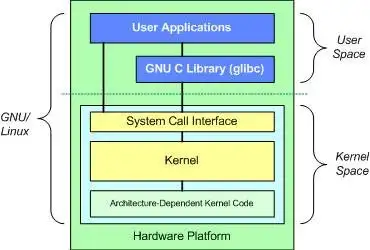
\includegraphics[width=0.8\textwidth]{img/core_gnu_linux.png}
\caption{Schema semplificato dell'interfaccia tra kernel, la libreria GNU C e le applicazioni dell'utente in un sistema operativo linux.}
\label{linux_core}
\end{figure}

\subsection{Distribuzioni Notevoli}
\begin{itemize}
	\item Red Hat Enterprise Linux (Server)\\
		Vi sono delle alternative Desktop, utilizzate spesso per testare nuove features e pacchetti prima di includerli nella versione Enterprise. Le maggiori in voga sono:
		\begin{itemize}
			\item Fedora
			\item CentOS
		\end{itemize}
	\item Debian (Desktop)\\
		Debian è un sistema operativo completamente libero, ed usa solo software e driver open source. Vi sono delle alternative, ad esempio Ubuntu, incentrata sull'utilizzo per utenti non esperit della riga di comando. Da Ubuntu sono derivate altre distribuzioni, come Mint, la quale è incentrata sulla leggerezza dell'interfaccia, oppure Kali, utilizzata per hacking e cyber security.
	\begin{itemize}
		\item Ubuntu
		\item Kali
		\item Linx Mint
	\end{itemize}
	\item Suse (Dektop / Server)\\
	L'alternativa a Red Hat per il mondo server. Come quest'ultimo, anche Suse è un sistema operativo modulare. Suse ha anche una controparte open source
	\begin{itemize}
		\item OpenSUSE
	\end{itemize}
	\item Arch Linux (Desktop)\\
	La distribuzione linux per eccellenza. Incentrata sul testing di nuove features del kernel linux e dei nuovi pacchetti. Arch Linux è il sistema operativo più malleabile e personalizzabile. Il contro è la modalità di installazione, che avviene solo tramite linea di comando. Da questa, sono derivate diverse distribuzioni, volte a ridurre la difficoltà di installazione di mantenimento. 
	\begin{itemize}
		\item Manjaro
		\item Garuda
		\item Endevour OS
	\end{itemize}
\end{itemize}

\chapter{Riga di Comando}
La riga dei comandi, o prompt dei comandi (CLI - Command Line Interface, Condole, Terminal, Shell) è la via più diretta per comunicare con il sistema operativo. I vantaggi sono:
\begin{itemize}
	\item E' semplice, ed a meno che non si commettono errori, funziona sempre.
	\item E' facile da programmare (rispetto alle applicazioni con interfaccia grafica (GUI))
	\item E' veloce nell'esecuzione dei comandi impartiti, ed efficiente nel gestire le risorse necessarie per far girare il programma.
\end{itemize}
Un altro grande vantaggio è che se il sistema operativo in qualche modo si rompe, la riga di comando è sempre accessibile (basta digitare Ctrl+Alt+F2 all'avvio del sistema operativo) attraverso quella che si chiama shell di login tty. Uno degli "svantaggi" è che bisogna conoscere i comandi. 
Ad esempio, se si vuole copiare un file in una cartella, si deve conoscere il comando di copia

\begin{verbatim}
 	cp nome_file_vecchio ~/cartella/nome_file_nuovo
\end{verbatim}
stessa cosa se si volesse creare una cartella

\begin{verbatim}
	mkdir nome_cartella
\end{verbatim}

La riga di comando può essere programmata attraverso degli script bash.\\
E' importante sapere sempre dove ci trova nella shell, o meglio sapere qual è la nostra \textit{working directory}. Dobbiamo anche sapere quali comandi verranno stoppati se chiudiamo la nostra shell.

\subsection{Elementi della shell}
Una volta aperta la shell \verb"tty"
, o un emulatore del terminale in linux, il prompt dei comandi si presenta nella forma:

\begin{verbatim}
	[username@login_shell ~] $
\end{verbatim}

dove lo user name è il nome dell'utente che ha effettuato il login sulla shell, e \verb"login_shell" è il nome con il quale il personal computer viene identificato nella rete locale, anche detto host name. Il simbolo \verb"~" identifica la \verb"home directory", che si trova in \verb"/home/nome_utente/home/". Per convenzione si utilizza il simbolo \verb"$" per identificare un utente standard, mentre \verb"#" per identificare un utente con privilegi di root. Un utente con privilegi di root può scrivere nelle cartelle diverse dalla home directory.\\
La struttura tipica di un comando \verb"bash" è la seguente
\begin{verbatim}
	[username@login_shell ~] $ hostname -f
\end{verbatim}
per eseguire il comando basta premere \verb"Enter" sulla tastiera. Tale comando stampa su schermo il nome del computer, l'output sarà dunque
\begin{verbatim}
	login_shell
\end{verbatim}
vediamo che accanto al comando \verb"hostname" viene aggiunta un'opzione \verb"-f". I comandi hanno tutti differenti opzioni, le quali possono essere stampate con l'ausilio del comando \verb"man", oppure aggiungendo l'opzione \verb"--help".\\
Una volta che il comando è stato eseguito, sarà di nuovo visibile il prompt di \verb"bash", dove sarà possibile digitare un nuovo comando. Finché non è stato eseguito un comando, non sarà possibile eseguire nessun altro comando, a meno che non si apra una nuova shell.\\
Possiamo navigare nella storia dei comandi della nostra shell utilizzando le frecce della tastiera, senza dover riscrivere il comando da capo. Se dobbiamo quindi eseguire più volte lo stesso comando possiamo cercarlo nella nostra \verb"bash_history".\\
Il tasto \verb"Tab" serve per l'autocompletamento (Tab completation) dei comandi. Se vogliamo che funzioni, dobbiamo scrivere abbastanza lettere per far si che il sistema operativo trovi il comando, che, come vedremo più in là sarà collegato ad un file binario all'interno di \verb"/usr/bin" o \verb"/usr/sbin". Premendo una seconda volta \verb"Tab" è possibile vedere una lista di comandi compatibili con le lettere già digitate nel prompt di \verb"bash". \\
L'ultima combinazione di tasti notevole è \verb"Ctrl-C", la quale ferma il comando che è attualmente in esecuzione. Questo fa si che il comando in esecuzione venga fermato con un messaggio di errore, spesso identificato come \verb"Keyboard Abort". \\
La riga di comando è sempre \textit{case sensitive}, ovvero fa differenza tra caratteri maiuscoli e minuscoli. Molto spesso le opzioni dei comandi possono essere scritte in più modi. Possiamo ad esempio scrivere
\begin{verbatim}
	sbatch --time 0:30:00
\end{verbatim}
oppure 
\begin{verbatim}
	sbatch -t 0:30:00
\end{verbatim}
questi due comandi sono identici. Il primo viene detto "full name command", mentre il secondo viene chiamato "shorthand command".\\
Uno svantaggio per gli utenti poco esperti della riga di comando è l'assenza totale del tasto \verb"Annulla". Ovvero, una volta mandato in esecuzione un comando non si può tornare indietro. Conseguentemente non vi saranno finestre di dialogo che chiedono se si è sicuri di voler procedere. Ad esempio, se vogliamo eliminare un file utilizzando il comando \verb"rm" la shell non ci chiederà se siamo sicuri di volerlo fare, e procederà con l'esecuzione del comando.\\
Questo potrebbe causare, nell'eventualità di utenti con permessi di root, gravi problemi se si eliminano o modificano files necessari al sistema operativo, ad esempio come\footnote{Mai mandare in esecuzione questo comando!}
\begin{verbatim}
 sudo rm -rf /
\end{verbatim}
Morale: mai mandare in esecuzione un comando se non si sa cosa esso faccia esattamente. 

\chapter{Struttura delle Cartelle in Linux}
\section{Struttura ad albero - Filesystem Tree}
Diversamente dai sistemi Windows, dove i volumi montati nel sistema (sia interni che esterni) sono etichettati da lettere (come ad esempio \verb"C:/"), su Linux esiste una sola root directory \verb"/". Il livello più alto di questo albero di cartelle è uguale in tutti i sistemi linux, ovvero è standardizzato. I volumi esterni e interni vengono montati in delle cartelle (spesso \verb"/mnt"), chiamati mounting points, ovvero punti di montaggio. Il percorso di un file può essere identificato in modo assoluto, ad esempio 
\begin{verbatim}
/home/nome_utente/Documenti/documento.pdf
\end{verbatim}
oppure in modo relativo sapendo quel è la working directory della nostra shell. Per sapere qual è la working directory si usa il comando \verb"pwd".

\begin{figure}
	\centering
	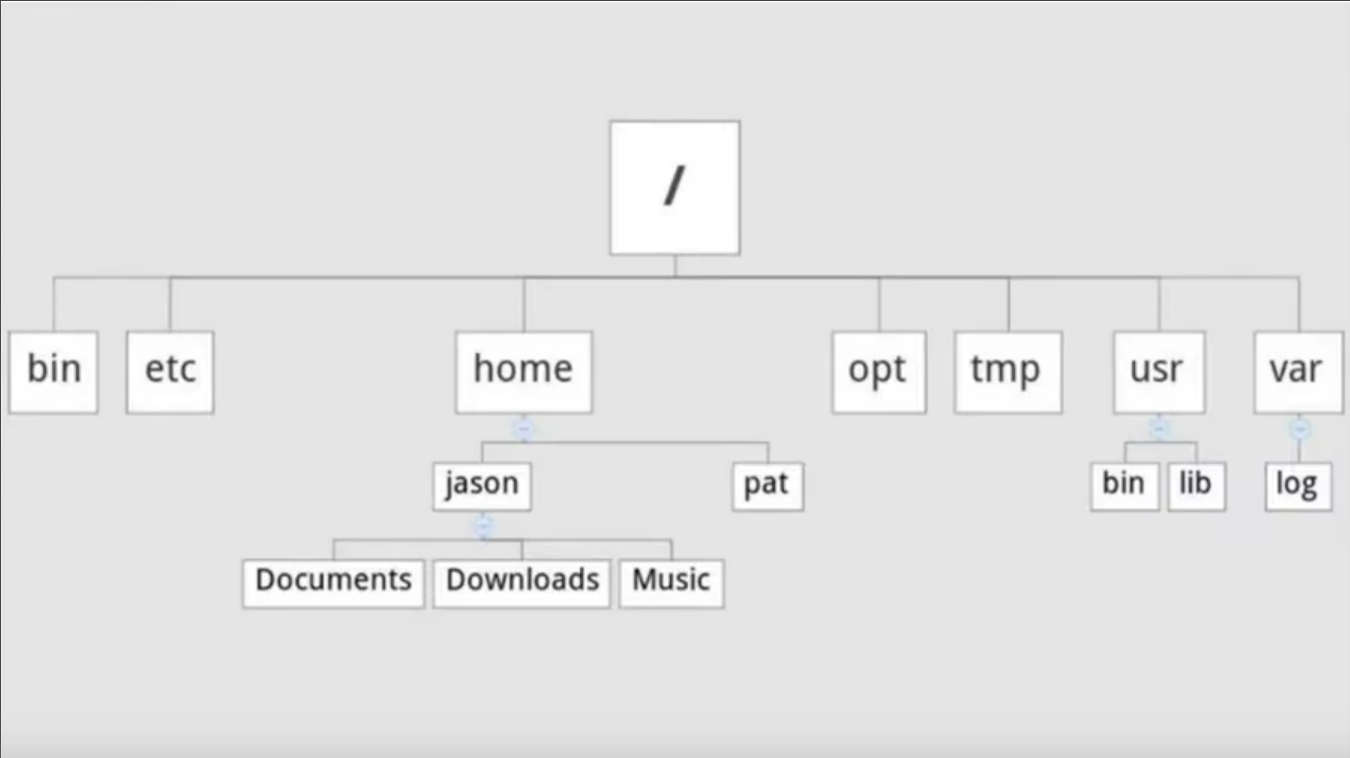
\includegraphics[width=0.8\textwidth]{img/filesystem_tree.png}
	\caption{Tipica struttura ad albero di un sistema Linux.}
	\label{fs_tree}
\end{figure}

Come vediamo nella Figura \ref{fs_tree} vi sono molte cartelle, che riassumiamo qui:
\begin{itemize}
	\item \verb"/": è la cartella di livello più alto, la quale contiene tutte le altre cartelle.
	\item \verb"bin/": qui vi sono tutti i programmi (come le shells, ad esempio)
	\item \verb"etc/": qui vi sono tutti i files di configurazione 
	\item \verb"home/": qui è dove l'utente spende la maggior parte del tempo. Vi sono tutti i files personali dell'utente, ed è l'unica cartella dove un utente non root può scrivere. Molte distribuzioni linux, tra le quali OpenSUSE, crea una partizione dedicata per questa cartella per aumentare la stabilità e la sicurezza del sistema. In questa cartella vi è una sottocartella per ogni utente del sistema.
	\item \verb"opt/": in questa cartella ci sono i programmi opzionali. Come vedremo, ad esempio in questa cartella potranno essere caricati driver opzionali (ad esempio quelli della scheda grafica, bluetooth, etc.) 
	\item \verb"tmp/": contiene i files temporanei utili ai programmi per poter girare. Ad esempio un estrattore di archivi zip può utilizzare questa cartella per contenere l'archivio da estrarre. 
	\item \verb"usr/": acronimo di "unix system resources", dove vi sono ancora altri programmi e librerie.
	\item \verb"var/": contiene dei files che cambiano nel tempo (variable files) come ad esempio i file di log, che possono essere consultati in caso di errore di esecuzione di qualche comando o programma.
\end{itemize}

Ogni cosa in linux è rappresentato sottoforma di file, molto spesso sotto forma di file di testo. Ad esempio, la configurazione di una shell grafica (ad esempio i3, gnome, kde) può essere configurata a partire da un file di configurazione senza passare per l'applicazione grafica che permette di personalizzare le impostazioni grafiche. Nel filesystem tree vi sono anche altre cartelle, il quale nome può variare a seconda della distribuzione. Ad esempio nella cartella \verb"/dev/" ci sono i files relativi ai dispositivi collegati alla scheda madre (ad esempio hard disks, pendirves, lettori DVD) mentre nella cartella \verb"/proc/" vi sono tutti i files relativi alle informazioni del sistema operativo.

Ogni comando che viene scritto nel prompt di bash è un programma o uno script, che giace in una cartella del filesystem. Per scoprire dove risiede tale programma o script basta scrivere
\begin{verbatim}
	which <comando>
\end{verbatim}
che darà come output
\begin{verbatim}
	/cartella/.../<comando>
\end{verbatim}
ad esempio se apriamo un shell bash e digitiamo il comando \verb"firefox", l'hostname command \verb"firefox" punterà al programma Firefox che aprirà una finestra con il browser internet. Vediamo alcune abbreviazioni per le cartelle nella shell di bash:
\begin{itemize}
	\item \verb"." indica la cartella corrente (working directory)
	\item \verb".." indica la cartella padre della cartella in cui siamo 
	\item \verb"~" indica la cartella \verb"/home/nome_utente/".
\end{itemize}

Per navigare nel filesystem si usa il comando \verb"cd", che sta per change directory, che è parte dello standard POSIX, ovvero è presente in tutti i sistemi linux / unix. Ad esempio con 
\begin{verbatim}
	cd ..
\end{verbatim}
ci spostiamo nella cartella padre della nostra attuale working directory. Notiamo che dopo il comando \verb"cd" vi è uno spazio, che delimita il comando dal suo argomento \verb".." ovvero la cartella di destinazione.\\
Un altro comando fondamentale è \verb"ls". Esso ci dice quali files giacciono in una specifica cartella. La sintassi è la seguente
\begin{verbatim}
	ls [OPTIONS] /percorso_cartella
\end{verbatim}
le opzioni di \verb"ls" sono molteplici. Le più importanti sono
\begin{itemize}
	\item \verb"-l" la quale ci fornisce più informazioni per i files all'interno della cartella. E' così comune che ha un suo link, ovvero un comando dedicato \verb"ll" = \verb"ls -l"
	\item \verb"-a" che ci fa vedere anche i files nascosti (i quali iniziano con un punto)
	\item \verb"-t" che ordina i files per data di modifica.
\end{itemize}


\subsection{Gestione dei Files}
Come prima cosa diciamo che negli ambienti Linux l'estensione del file non importa. L'estensione viene utilizzata per facilitare la lettura da parte degli utenti. Qualche programma potrebbe cercare l'estensione dei file, ma sono casi rari. Ciò che importa al sistema è se un file sia di testo o meno. Esempi di file di testo sono
\begin{itemize}
	\item File di configurazione
	\item Scripts e programmi (\verb".sh", \verb".c", \verb".cpp", \verb".p")
	\item File di informazione del sistema
\end{itemize}
L'altra grande categoria di files sono i files binari. Questi non possono essere cercati ne letti (ad esempio con il comando \verb"cat" o \verb"more"). Ci viene in aiuto il comando \verb"file", il quale ci indica il tipo di file. \\
Ad esempio, se abbiamo un file di testo che abbiamo denominato \verb"test.jpeg" e digitiamo
\begin{verbatim}
	file test.jpeg
\end{verbatim}
l'output sarà
\begin{verbatim}
	test.jpeg: ASCII text
\end{verbatim}
ovvero il file \verb"test.jpeg" è un file di testo codificato con codice \verb"ASCII". Per un'immagine vera, l'output sarà diverso, ad esempio:
\begin{verbatim}
	JPEG image data, Exif standard: [TIFF image data, little-endian, 
\end{verbatim}
\begin{verbatim}
	direntries=0], baseline, precision 8, 3840x2160, components 3
\end{verbatim}

Molti dei comandi che manipolano i files, funzionano anche per le cartelle, delle volte basta aggiungere l'opzione \verb"-r" che sta per \verb"--recursive". Nei casi più semplici, come ad esempio il comando \verb"mv" che sposta/rinomina i files e le cartelle non è necessario aggiungere l'opzione \verb"-r". 
\begin{verbatim}
	mv <vecchio_nome> <nuovo_nome>
\end{verbatim}

Un altro comando fondamentale è quello utilizzato per copiare i files
\begin{verbatim}
	cp <vecchio_nome> <nuovo_nome>
\end{verbatim}
Se vogliamo copiare un'intera cartella basta aggiungere l'opzione \verb"-r":
\begin{verbatim}
	cp -r <vecchia_cartella> <nuova_cartella>
\end{verbatim}

Per creare un file vuoto si utilizza il comando \verb"touch":
\begin{verbatim}
	touch nome_file
\end{verbatim}
questo viene utilizzato anche per accedere al file e modificare dunque la data di accesso ad un file. \\
D'altra parte esiste anche un comando utilizzato per rimuovere un file o una cartella. 
\begin{verbatim}
	rm <nome_file>
	rm -r <nome_cartella>
\end{verbatim}

E' possibile utilizzare anche l'opzione \verb"-f" che sta per \verb"--force", che fa sì che la shell non ci chieda ogni volta se siamo sicuri di eliminare il suddetto file. \\
Tutti questi comandi funzionano con un solo file. Possiamo passare come argomenti più files, oppure
\begin{itemize}
	\item Globbing \verb"?" per il numero di caratteri che mancano. Ad esempio se abbiamo dei files nella nostra cartella
	\begin{verbatim}
		file1.txt file2.txt file3.txt file4.txt file11.txt
	\end{verbatim}
	e digitiamo 
	\begin{verbatim}
		rm file?.txt
	\end{verbatim}
	esso rimuoverà tutti i files tranne \verb"file11.txt".
	\item Globbing \verb"*". Digitando invece
	\begin{verbatim}
		rm file*.txt
	\end{verbatim}
	verranno rimossi tutti i files.
	\item Globbin \verb"[]". Digitando 
	\begin{verbatim}
		rm file[1-3].txt
	\end{verbatim}
	verranno rimossi tutti i files tranne \verb"file4.txt" e \verb"file11.txt".
\end{itemize}

Se vogliamo cercare un file possiamo utilizzare il comando \verb"find". Ad esempio digitando 
\begin{verbatim}
	find . -name "file1.txt" -type f
\end{verbatim}
cerchiamo un file nella cartella \verb".", ovvero la nostra working directory denominato \verb"file1.txt" di tipo \verb"f" ovvero file. Se cerchiamo una directory l'opzione da aggiungere sarà \verb"-type d".\\
Possiamo scegliere tante opzione, le quali rendono questo comando molto potente. Possiamo ad esempio cercare dei file che sono stati modificato solo dopo un certo tempo, oppure eseguire un comando per ogni file che viene trovato (opzione \verb"-exec"). Le wildcards, ovvero i caratteri \verb"? * []" introducono dei problemi nella shell. Infatti, può capitare che passando un argomento come ad esempio \verb"file*.txt" si raggiunga il limite massimo degli argomenti passabili al comando. Questo succede perché la shell prima crea una lista di argomenti con tutti i possibili nomi associati a \verb"file*.txt" e poi li passa come argomento al comando. Per ovviare a questo problema, ad esempio nel comando \verb"find" si può utilizzare l'identificatore di stringa (\verb""""):
\begin{verbatim}
	find . -type f -name "file*.txt"
\end{verbatim}
in questo modo non è la shell che crea la lista di argomenti, ma se ne occupa il comando \verb"find". 

\section{Canali I/O}
La shell bash ha fondamentalmente tre modi per comunicare con l'utente:
\begin{itemize}
	\item Standard input (\verb"stdin"): cosa scriviamo nel prompt della shell
	\item Standard output (\verb"stdout"): output normale della shell
	\item Standard error (\verb"stderr"): output di errore della shell
\end{itemize}
E' molto comodo separare i canali di output. Un canale, o stream, è un deposito di memoria dal quale escono i dati di output (che andranno nei due canali di output \verb"stdout" e \verb"stderr", e riceve dati dal canale di input \verb"stdin"). 

Lo standard input è un canale da cui giunge un flusso di dati (spesso testuali) in ingresso ad un programma. Il programma li trasferisce effettuando operazioni di lettura. Non tutti i programmi necessitano di dati in input: ad esempio i comandi ls o dir (che mostrano il contenuto delle directory) svolgono il loro compito senza bisogno di leggere dati in input.
Il flusso di input, salvo casi di redirezione\footnote{Deviazione dei canali standard (standard input, standard output e standard error) di un dato comando verso destinazioni (o da sorgenti, nel caso dello standard input) che sono diverse da quelle predefinite.}, proviene dal terminale (es. dall'utente tramite tastiera) da cui il programma è stato avviato. 

Lo standard output è il canale su cui un programma scrive i suoi dati in output. Il programma trasferisce i dati effettuando operazioni di scrittura. Non tutti i programmi producono output: ad esempio il comando mv (che cambia il nome di un file o di una directory) normalmente non produce dati in output.
Il flusso di output, salvo casi di redirezione, è diretto al terminale da cui il programma è stato avviato (es. a monitor o console a favore dell'utente). 

\begin{figure}
	\centering
	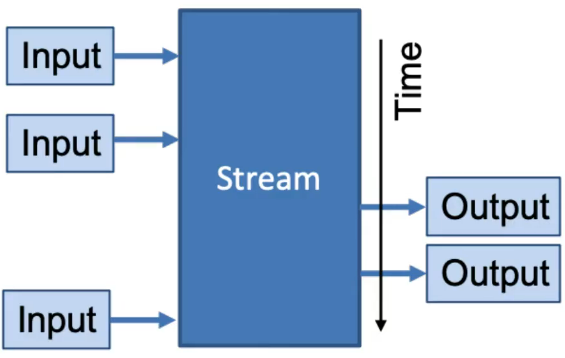
\includegraphics[width=0.8\textwidth]{img/streams.png}
	\caption{Schematizzazione semplificata di un canale.}
	\label{fig:streams}
\end{figure}

Lo standard error è un altro canale di output, tipicamente usato dai programmi per i messaggi d'errore o di diagnostica. Esso è un canale indipendente dallo standard output, e se ne può effettuare la redirezione separatamente dagli altri. La sua destinazione è solitamente il terminale da cui il programma è stato avviato, in modo da rendere massime le possibilità di essere visto anche quando lo standard output è diretto altrove: ad esempio, nel caso di una pipeline software, l'output di un programma è fornito come input al programma successivo, ma i suoi messaggi d'errore sono ancora visualizzati sul terminale.
È accettabile e normale che lo standard output e lo standard error abbiano la stessa destinazione, come nel caso del terminale testuale: i messaggi compaiono nello stesso ordine in cui il programma li scrive, salvo quando sono in uso dei buffer (ad esempio quando lo standard error non ha buffer e lo standard output ha un buffer di linea: in questo caso i dati scritti sullo standard error in un secondo momento possono apparire prima dei dati scritti su standard output in un primo momento, in quanto il buffer dello standard output potrebbe non essere ancora stato riempito). 

Come vediamo in Figura \ref{fig:streams} l'input e l'output possono talvolta sovrapporsi, e non ci sono regole che gestiscono l'ordine in cui avvengono l'input e l'output. 

Possiamo inoltre redirezionare l'input e output ad altre sorgenti. Possiamo ad esempio redirezionare l'input di un comando e prenderlo dall'output di un altro comando, oppure possiamo redirezionare l'output in uno stream su file con la sintassi:
\begin{verbatim}
	comando > file
\end{verbatim} 

Con il simbolo \verb">" possiamo infatti redirezionare lo \verb"stdout" su un file denominato \verb"file". Per redirezionare lo \verb"stdout" si usa la sintassi

\begin{verbatim}
	comando 2> file
\end{verbatim}

mentre se vogliamo dare in input ad un comando un file, e quindi redirezionare lo \verb"stdin" si usa
\begin{verbatim}
	comando < file
\end{verbatim}

Possiamo poi, come già detto, utilizzare l'output di un comando (\verb"comando2") come input di un altro comando (\verb"comando1") utilizzando il simbolo pipe \verb"|":
\begin{verbatim}
	comando1 | comando2
\end{verbatim}

Potremmo aver bisogno di appendere output di più comandi sullo stesso file senza sovrascriverlo ogni volta. Per fare questo si utilizza il simbolo \verb">>":
\begin{verbatim}
	comando >> file
\end{verbatim}

Nei sistemi Linux, i canali I/O standards sono numerati seguendo la convenzione del linguaggio C. \begin{verbatim}
	0: stdin
	1: stdout
	2: stderr
\end{verbatim}
Potremmo voler redirezionare lo \verb"stdout" di un programma in un file diverso dal canale \verb"stderr". 
\begin{verbatim}
	comando > output.log 2> error.log
\end{verbatim}
Con questa sintassi si redireziona lo standard output nel file \verb"output.log" mentre lo standard error in \verb"error.log". Possiamo inoltre redirezionare entrambi i canali sullo stesso file con la sintassi

\begin{verbatim}
	comando 2>&1 > output_error.log
\end{verbatim}

\subsection{Visualizzazione e Ricerca}
Vediamo ora alcuni comandi per la visualizzazione del contenuto di un file di testo sulla console bash. Per visualizzare il contenuto di un file esistono diversi modi. Il più semplice è l'utilizzo del comando \verb"cat". Con il comando \verb"less" inoltre possiamo scorrere il testo (ad esempio il comando \verb"man" usa questo comando per visualizzare il file di testo nel quale vengono spiegati i vari utilizzi dei programmi). Altri comandi, come ad esempio \verb"head" o \verb"tail" stampano in \verb"stdout" le prime righe o le ultime di un file.\\
Il comando \verb"grep" viene utilizzato per la ricerca di contenuti nei file di testo. La sintassi è
\begin{verbatim}
	grep [OPZIONI] [stringa da cercare] [nome del file]
\end{verbatim} 
ad esempio

\begin{verbatim}
	grep -i -r "test" example*.txt
\end{verbatim}
le opzioni più comuni sono
\begin{verbatim}
	-r: ricerca ricorsiva
	-i: ignora maiuscole e minuscole
	-I: ignora i file di tipo binario
\end{verbatim}

Questo comando è molto utile quando ci ritroviamo con dei files di grandi dimensioni e vogliamo cercare una specifica stringa all'interno di esso. Come il comando \verb"find", a causa delle wildcards e la moltitudine di opzioni, è molto potente. \\
Possiamo utilizzare il comando \verb"grep" combinandolo con il comando \verb"ll" (ovvero \verb"ls -l") usufruendo del simbolo pipe \verb"|" con questa sintassi:
\begin{verbatim}
	ll | grep -i test
\end{verbatim}
questo comando fa vedere tutti i files che hanno al loro interno una stringa \verb"test".

\chapter{Utenti e Processi}
Come ogni sistema operativo moderno, anche Linux è un sistema multiutente. Questo vuol dire che il login nel sistema operativo può essere effettuato da più utenti. Esistono fondamentalmente due tipologie di utente: standard o amministratore. Ogni utente, nei sistemi Linux possiede una cartella \verb"home" dedicata. \\

\section{Permessi}
L'accesso ai files di sistema viene regolamentato attraverso dei \verb"permessi" specifici per ogni utente. Solo l'utente \verb"root" può fare qualsiasi cosa all'interno del sistema operativo. Ad esempio ad un utente standard potrebbe essere persino impedito di leggere in alcune cartelle. Questi permessi possono essere configurati solo dagli utenti amministratori. \\
Ogni file ed ogni cartella ha specifici permessi. Tali regole specificano cosa può fare o non fare con quel file o quella cartella\footnote{"Non puoi rompere ciò che non vedi".}.\\
Gli utenti standard, nel caso in cui conoscano la \verb"password" dell'amministratore, possono ottenere i permessi di \verb"root" e lanciare programmi o comandi con tali permessi digitando
\begin{verbatim}
	sudo <comando>
\end{verbatim}

Ogni utente appartiene a uno o più gruppi. Non appena viene creato, un utente appartiene ad un gruppo primario. Anche in base a quest'appartenenza si possono configurare i permessi per i files e cartelle. Esistono tre tipi di permessi:
\begin{itemize}
	\item Lettura (\verb"r"): chi può vedere il contenuto di files e cartelle
	\item Scrittura (\verb"w"): chi può cambiare il contenuto di files e cartelle
	\item Esecuzione (\verb"x"): chi può eseguire un file (ad esempio uno script bash \verb".sh")
\end{itemize}

Questi tre tipi di permessi di files non sono indipendenti. Ovviamente per poter modificare un file deve essere necessario vederli. Quindi in molti casi, se non tutti, il permesso di scrittura include quello di lettura. E' possibile però poter eseguire uno script senza essere in grado di leggere il suo contenuto. \\
Per poter vedere chi ha il permesso su un file, chi lo ha creato, e quali permessi hanno i gruppi, etc. si utilizza il comando \verb"ll".

\begin{figure}
	\centering
	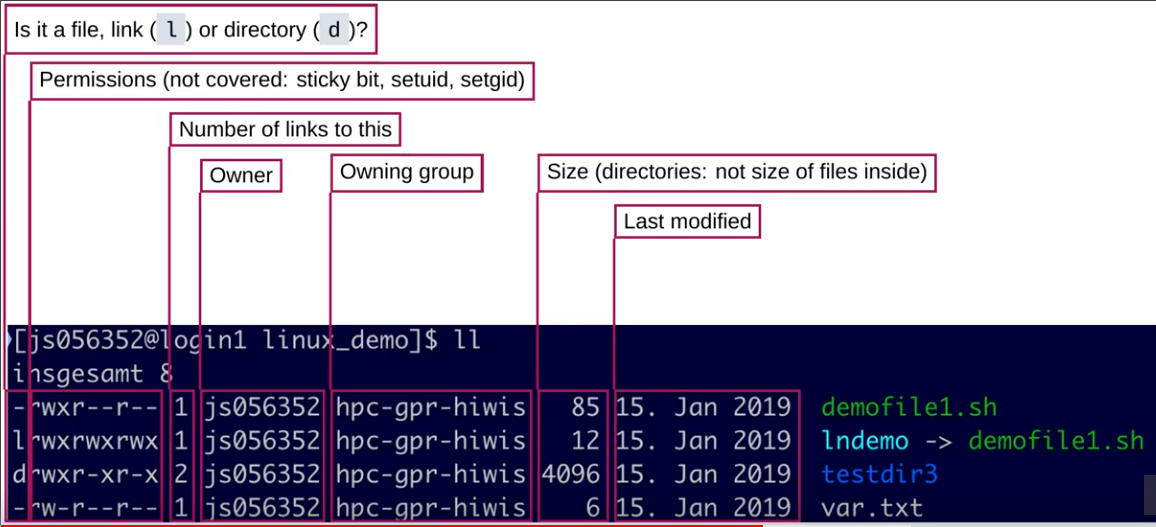
\includegraphics[width=0.8\textwidth]{img/permessi.png}
	\caption{Output del comando ll.}
	\label{llcommand}
\end{figure}

Vediamo più in dettaglio l'output introdotto in Figura\ref{llcommand}
\begin{verbatim}
	drwxr-xr-x 2 user groups size data_ultima_modifica nome_file
	-rw-r--r-- 1 user groups size data_ultima_modifica nome_file
\end{verbatim}
la prima lettera (prima riga \verb"d", seconda riga \verb"-") indica il tipo di file. 
\begin{verbatim}
	d: directory
	f: file
	-: not set
	l: link
\end{verbatim}
poi abbiamo tre sequenze di \verb"rwx". La prima di queste ci indica i permessi che possiede l'utente \verb"user" sul file o cartella. La seconda sequenza indica i permessi dei gruppi \verb"groups" che possiedono il file. La terza sequenza indica quali permessi degli utenti di altri gruppi che non possiedono il file. Nella seconda riga vediamo che alcuni permessi non ci sono. Quando un utente o un gruppo non ha un permesso, esso viene visualizzato con il simbolo \verb"-".
\subsection{Cambiare i permessi}
Esistono dei comandi volti a cambiare i permessi di files/cartelle, e la modifica del possessore di quest'ultimi. Con il comando \verb"chown" si può cambiare il possessore di un file. Esso necessita di permetti di \verb"root":
\begin{verbatim}
	sudo chown <nuovo_possessore> <nome_file>
	sudo chown <nuovo_possessore>:<nuovo_gruppo> <nome_file>
\end{verbatim}

Per cambiare i permessi di un file, possiamo utilizzare il comando \verb"chmod" con la seguente sintassi di esempio:
\begin{verbatim}
	chmod u+x <nome_file>
\end{verbatim}
dobbiamo quindi specificare tre opzioni. La prima specifica per "chi" cambiare il permesso, ed abbiamo quattro possibilità
\begin{verbatim}
	u: user
	g: group
	o: others
	a: all
\end{verbatim}
La seconda opzione specifica se aggiungere (\verb"+") o togliere (\verb"-") il permesso, mentre la terza deve specificare quale permesso \verb"r", \verb"w", oppure \verb"x".

\section{Gestione dei Processi}
In Linux, un file eseguibile memorizzato su disco costituisce un programma. Quando un programma viene lanciato e caricato in memoria viene chiamato processo. Con linguaggio tecnico possiamo definire il processo come l'istanza di un programma.\\
I processi hanno un ciclo vitale simile a quello degli organismi viventi: nasce (il programma viene lanciato), vive (il programma è in esecuzione) e muore (il programma viene terminato).\\
Esistono tre tipi di processi:
\begin{itemize}
	\item Processi di sistema (\verb"system"), anche detti demoni (\verb"daemons")
	\item Processi dell'utente (\verb"user")
	\item Processi dell'utente manuali (\verb"user manually launched")
\end{itemize}

I primi sono i processi necessari al sistema operativo per essere in esecuzione (ad esempio il processo che gestisce un driver). La seconda tipologia indica i processi dell'utente necessari per l'avvio di altri processi (ad esempio il gestore delle finestre, o window manager (\verb"wm"))
Possiamo visualizzare sulla shell di bash i processi attualmente in esecuzione con il comando \verb"top". Altri comandi danno delle specifiche differenti sui processi, come ad esempio \verb"pstree", il quale ci indica l'albero delle dipendenze dei processi. Ad esempio, lanciando il browser web \verb"firefox", esso ha bisogno che sia attivo il processo che gestisce le finestre, in quanto \verb"firefox" è un browser web grafico. \\

\begin{figure}
	\centering
	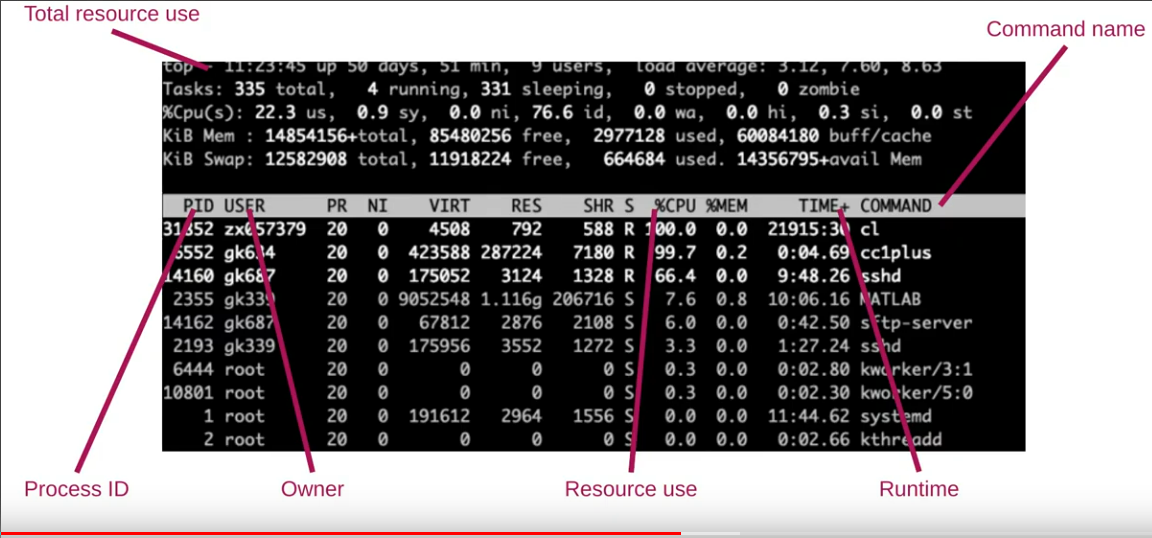
\includegraphics[width=0.8\textwidth]{img/top.png}
	\caption{Tipico output del comando top.}
	\label{top_out}
\end{figure}
Come per i file e le cartelle, anche i processi hanno un possessore. Solo il possessore del processo può cambiarne lo stato. Ad esempio, sapendo che il gestore delle finestre è posseduto dall'utente \verb"root", solo chi conosce la password di \verb"root" può lanciare o chiudere il gestore. In generale vale la regola che un processo può fare solo quello che il suo possessore può fare. Ad esempio un programma, che lanciato diventa un processo, non può scrivere in una cartella in cui il possessore del processo non ha il permesso di scrittura.\\
Quando viene avviato un processo gli viene assegnato un numero univoco chiamato ID processo (\verb"PID") che lo identifica in modo univoco nel sistema.
Il \verb"PID" non è modificabile e non varia per tutta la durata del processo. Solitamente il valore di \verb"PID" viene assegnato in modo sequenziale: un nuovo processo, quindi, assumerà un valore di \verb"PID" maggiore di uno rispetto all'ultimo processo creato.\\
Conoscendo il \verb"PID" è possibile agire sul processo, ad esempio terminandolo.
Il programma \verb"top" ha diversi comandi
\begin{itemize}
	\item \verb*|u|: filtra i processi in base all'utente che li possiede
	\item \verb*|k|: uccide uno specifico processo
	\item \verb*|h|: mostra i comandi (identico a \verb*|--help|)
	\item \verb*|f|: gestisce le colonne mostrate da \verb*|top|
	\item \verb*|x|: sottolinea e ordina secondo una colonna
	\item \verb*|<>|: sceglie la colonna secondo la quale ordinare i processi
	\item \verb*|R|: inverte l'ordine della colonna selezionata
	\item \verb*|q|: esce da \verb*|top|
\end{itemize}

Abbiamo già visto che un comando lanciato dalla shell diventa un processo. Lanciando solamente il programma, esso verrà eseguito nella shell, e terrà la shell occupata fino alla fine dell'esecuzione dello stesso. Digitando invece
\begin{verbatim}
	<comando> &
\end{verbatim}
esso verrà eseguito in background. Questa sintassi ci è utile se il programma viene eseguito su una finestra. In questo modo, infatti, la shell continuerà ad essere utilizzabile. \\
Possiamo sospendere un comando che è stato mandato nella shell utilizzando la combinazione da tastiera \verb*|Ctrl+z|. Un comando che è stato messo in pausa può essere mandato in background utilizzando il comando \verb*|bg|. Possiamo inoltre riportare nella shell un comando che è stato messo in background con il comando \verb*|fg|, con la sintassi
\begin{verbatim}
	fg <job-ID>
\end{verbatim}
dove il \verb*|job-ID| è diverso dal \verb*|PID|, e può essere visualizzato con il comando \verb*|jobs|.

\chapter{Strumenti e Utilities}

\section{L'editor di testo VIM}
L'editor di testo predefinito di Linux si chiama \verb*|vi|. Questo ha anche una versione migliorata: \verb*|vim| (\verb*|vi| improved). Esso è un editor da console, ovvero non viene lanciata una finestra grafica, ma il file viene editato direttamente all'interno della shell bash.\\
Tra i vantaggi troviamo
\begin{itemize}
	\item Sempre disponibile, in tutti i sistemi Linux 
	\item A patto di conoscerne i comandi, è molto efficiente e veloce.
\end{itemize}
Mentre abbiamo lo svantaggio di avere un interfaccia utente molto poco intuitiva, e la mole di comandi disponibili è eccessiva. 

\begin{figure}
	\centering
	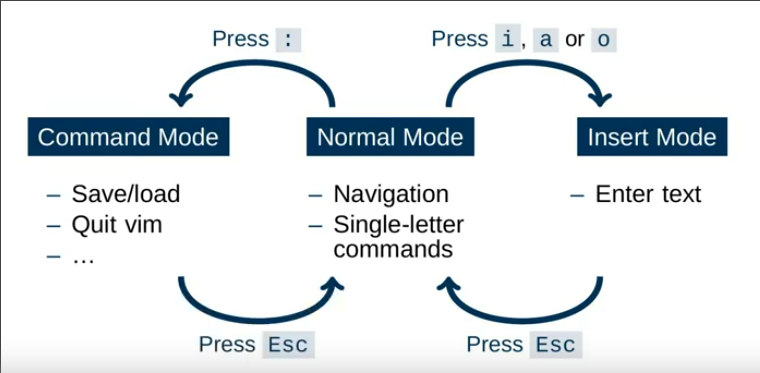
\includegraphics[width=0.8\textwidth]{img/vim_modes.png}
	\caption{Schema di comandi per cambiare la modalità di vim.}
	\label{vim_modes}
\end{figure}
Da \verb*|vi| mantiene la caratteristica di essere modale, ovvero di avere modalità diverse nelle quali i normali caratteri della tastiera hanno significato di inserimento testo o di comandi. In questo modo, è possibile usarlo senza far uso del mouse, né dei tasti meta, permettendo una velocità maggiore di scrittura, a prezzo di maggiore difficoltà di utilizzo da parte di nuovi utenti. Vediamo qui di seguito alcuni dei comandi più comuni. Per aprire un file vuoto si utilizza il comando \verb*|vim|, mentre per aprire un file con uno specifico nome
\begin{verbatim}
	vim <nome_file>
\end{verbatim}
 I comandi più comuni sono:
 \begin{itemize}
 	\item Gestione file:
 		\begin{itemize}
 			\item \verb*|:w| per salvare il file (\verb*|write|)
 			\item \verb*|:w <nome_file>| per salvare il file con nome \verb*|<nome_file>|
 			\item \verb*|:wq|, \verb*|:x|, \verb*|ZZ| per salvare e chiudere
 			\item \verb*|:q!| per chiudere il file senza salvare.
 		\end{itemize}
 	\item Muoversi all'interno del file:
 		\begin{itemize}
 			\item \verb*|frecce| per muovere il cursore nella direzione della freccia
 			\item \verb*|h,j,k,l| per muovere il cursore a sinistra, giù, su, destra
 			\item \verb*|$| per muovere il cursore alla fine del file
 			\item \verb*|gg| per muovere il cursore alla prima riga
 			\item \verb*|G| per muovere il cursore all'ultima riga
 			\item \verb*|w| per saltare alla parola successiva
 			\item \verb*|b| per saltare alla parola precedente
 			\item \verb*|%| per saltare al carattere corrispondente, ad esempio \verb*|(...),[...],{...}|
 		\end{itemize}
 	\item Modifica del testo:
 		\begin{itemize}
 			\item \verb*|u|: annulla l'ultima modifica
 			\item \verb*|Ctrl + r|: rifai l'ultima modifica
 			\item \verb*|.|: ripeti l'ultimo comando
 			\item \verb*|x|: cancella carattere
 			\item \verb*|dd|: elimina l'intera riga
 			\item \verb*|yy| o \verb*|Y|: copia l'intera riga
 			\item \verb*|p|: incolla contenuto dopo il cursore
 		\end{itemize}
 	\item Ricerca:
 		\begin{itemize}
 			\item \verb*|/pattern|: vai avanti nella ricerca per espressioni regolari
 			\item \verb*|?pattern|: vai indietro nella ricerca espressioni regolari
 			\item \verb*|n|: ripeti l'ultima ricerca
 			\item \verb*|N|: ripeti l'ultima ricerca nella direzione opposta
 			\item \verb*|%s/old/new/|: sostituisce \verb*|old| con \verb*|new| nella riga corrente
 			\item \verb*|%s/old/new/g|: sostituisce \verb*|old| con \verb*|new| nell'intero file		
 		\end{itemize}
 \end{itemize}


\section{Shell Scripts}
Una volta che sappiamo come interagire con la la shell di Linux, sappiamo anche dare una serie di istruzioni, e salvare queste in un file eseguibile. Questi sono detti \textit{scripts}. Questo file di testo viene dato in input nel terminale, ed esso eseguirà tutte le istruzioni contenute al suo interno. Il vantaggio di questo metodo di scripting è ovviamente l'automazione di alcune operazioni che viene fatta molto semplicemente scrivendo le istruzioni. Lo svantaggio, se così si può dire, è che non sappiamo della presenza di errori fino al momento in cui lo script non viene lanciato nel terminale. \\
Per eseguire uno script \verb*|.sh| basta scrivere nel terminale:
\begin{verbatim}
	./script.sh
\end{verbatim}
avendo cura che l'utente abbia il permesso di eseguire il file nella shell.\\
Come vediamo dalla sintassi, dobbiamo specificare in che cartella si trova il nostro script, infatti nel nostro caso abbiamo identificato la working directory con \verb*|./|. Questo perché Linux cerca i comandi nella cartella in cui siamo, al massimo nelle directories incluse nella variabile di ambiente della \verb*|$PATH|\footnote{Approfondiremo il concetto e gli utilizzi delle variabili d'ambiente successivamente.} per questioni di sicurezza. Vediamo un primo esempio di script bash.
\begin{esempio}
	\begin{verbatim}
		\\
		1 #!/bin/bash
		2
		3 #Questo è un commento
		4 echo "Hello World"
		5
		6 ls -l
		7 sleep 3s
		8 ls \
		9  -l
	\end{verbatim}
\end{esempio}

Nella riga \verb*|1| viene specificato l'interprete di \verb*|bash|. Questa direttiva deve trovarsi sempre nella prima riga di ogni script. Esso si specifica con il carattere utilizzato per i commenti, \verb*|#| seguito dal punto esclamativo \verb*|!|. Vediamo che alla riga \verb*|8| c'è il simbolo \verb*|\|. Esso specifica che il comando continua a capo. \\
Durante l'esecuzione degli script verrà stampato sulla console l'output di tutti i comandi. Utilizzando le redirezioni possiamo, ovviamente, stampare su file tali output. \\
Possiamo assegnare un valore ad una variabile tramite l'operazione binaria \verb*|=|. 
\begin{verbatim}
	var="valore"
\end{verbatim}
dove notiamo che ai lati del simbolo \verb*|=| non vi sono spazi. I simboli \verb*|"..."| servono quando nel valore vi sono degli spazi o dei caratteri speciali. \\
Possiamo stampare il valore di \verb*|var| con
\begin{verbatim}
	echo $var
\end{verbatim}	
Un errore comune che viene commesso durante l'assegnazione delle variabili è confondere il ruolo delle doppie virgolette e quello delle singole virgolette.\\
Utilizzando le singole virgolette verrà assegnata alla variabile il contenuto esatto. Ad esempio scrivendo:
\begin{verbatim}
	var='$ciao'
\end{verbatim}
nella variabile \verb*|var| ci sarà la stringa \verb*|$ciao|, mentre usando
\begin{verbatim}
	var1='ciao'
	var2="$var1"
\end{verbatim}
nella variabile \verb*|var2| ci sarà il valore effettivo di \verb*|var1|, che è in questo caso la stringa \verb*|ciao|. Se racchiudiamo tra parentesi un comando, esso verrà primo eseguito. Ad esempio digitando
\begin{verbatim}
	var=$(bla)
\end{verbatim}
verrà prima eseguito il comando \verb*|bla| e il suo output verrà memorizzato nella variabile \verb*|var|.\\
Possiamo passare degli argomenti quando eseguiamo lo script dal terminale. Ad esempio digitando:
\begin{verbatim}
	./script.sh -f 5.0
\end{verbatim}
nello script avremo le seguenti variabili assegnate
\begin{verbatim}
	$0=script.sh
	$1=-f
	$2=5.0
\end{verbatim}
Possiamo inoltre usufruire dei ciclo e degli statements \verb*|if|
\begin{esempio}
	\begin{verbatim}
		#!/bin/bash
		for file in $( ls ); do
			echo item: $file
		done
		
		if[ -e $filename ]; then
			echo "$filename exists."
		fi
	\end{verbatim}
\end{esempio}



\chapter{Variabili di Ambiente}
Le variabili d'ambiente, nei sistemi Unix-like, e più in generale negli ambienti \verb*|POSIX| sono delle variabili specifiche per ogni processo. Ogni processo possiede il proprio insieme di variabili d'ambiente distinto e separato da quello degli altri processi, ed in nessun caso un processo può modificare le variabili d'ambiente di un altro processo; esse tuttavia si propagano, duplicandosi, di processo padre in processo figlio. \\
Le variabili d'ambiente hanno un ruolo tradizionalmente significativo nella configurazione dei programmi: esse sono usate ad esempio per specificare le impostazioni di localizzazione, o per indicare ad un programma le directory ove reperire le proprie risorse, o ancora per modificarne il comportamento predefinito. \\
\section{Caratteristiche}
Possiamo assegnare una variabile di ambiente ad un processo\footnote{Ogni processo ha la sua lista di variabili che possiamo assegnare.} o direttamente alla shell. Ad esempio, per la console del terminale la variabile di ambiente \verb*|HOME| si può stampare su schermo con il comando:
\begin{verbatim}
	echo $HOME
\end{verbatim}
che darà come risultato
\begin{verbatim}
	/home/nome_utente
\end{verbatim}

Le variabili di ambiente sono molto utili per la creazione di script, in quanto possiamo modificare le cose localmente. Ad esempio è possibile impostare percorsi differenti per librerie diverse. Supponiamo di voler lanciare un codice con alcune librerie su due diverse architetture di processori. Grazie alle variabili di ambiente possiamo configurare le librerie che il nostro codice utilizza prima della compilazione, in questo modo se andiamo a compilare il nostro codice su un'architettura \verb*|arm64| o \verb*|amd64|, non dobbiamo cambiare il codice, ma solamente il percorso delle librerie che saranno differenti per ogni architettura.\\

Molte variabili di ambiente vengono inizializzate quando il sistema operativo viene installato, ad esempio la variabile \verb*|HOME| che abbiamo visto prima, oppure la variabile \verb*|USER|, mentre alcune variabili di ambiente vengono assegnate quando installiamo del software, ad esempio delle librerie grafiche, o il compilatore \verb*|gcc/g++|.\\
Per visualizzare tutte le variabili di ambiente impostate basta utilizzare il comando \verb*|env|. Per crearne una nuova, si utilizza la convenzione di definirle in maiuscolo, ad esempio:
\begin{verbatim}
	export MY_VAR="value"
\end{verbatim}

D'ora in poi la variabile \verb*|MY_VAR| sarà disponibile nei processi figlio. 

\subsection{Moduli di Ambiente}
In un contesto cluster, è molto probabile, data la mole di utenti con differenti esigenze, che siano necessarie diverse versioni dello stesso software. Un esempio è il modulo \verb*|OpenMPI|. Per adattarsi alle differenti esigenze, potrebbe essere necessario utilizzare una o l'altra versione dello stesso compilatore. Per risolvere il problema, si possono costruire più ambienti, dove le variabili assumono valori diversi. Questo viene fatto perché in linea di principio un amministratore del sistema non sa cosa serve all'utente, e quindi è meglio dare la possibilità di caricare diverse versioni dello stesso modulo. Ad esempio:
\begin{verbatim}
	module load openmpi/gcc/64/1.10.3
\end{verbatim}
carica il modulo \verb*|OpenMPI| compilato con \verb*|gcc| per sistemi \verb*|x64| nella versione \verb*|1.10.3|. \\
Ad ogni modulo viene generalmente associato un file di definizione, che può essere uno script \verb*|LUA|\footnote{\hyperref{https://www.lua.org/}{docu}{LUA}{Documentazione LUA}} o \verb*|Tcl|\footnote{\hyperref{https://www.tcl.tk/}{docu}{tcl}{Documentazione Tcl}}.


\section{Esempi di utilizzo}

\section{Variabili di Ambiente notevoli}






\end{document}